\chapter{Visualizing Dynamic Input Graphs}
\label{chap:visualizing-dynamic-input-graphs}

Extending the approach discussed in the previous section to dynamic input graphs is challenging primarily because we must try to preserve the viewer's mental map as the underlying data changes over time. We want the visualization at different points in time to be similar enough so that the viewer can clearly tell what parts have changed \cite{mashima2011visualizing}, yet allow for the required changes in geography and topology. Still, changes between visualizations of consecutive points in time should minimize movement and allow for smooth animations therebetween.

The pipeline for static inputs discussed in the previous section does not satisfy these requirements. Running through the entire pipeline with a different, albeit similar, input graph, may result in a completely different visualization, destroying the viewer's mental map: The filtering \& embedding and transformation phases in particular have way too many degrees of freedom in choosing which edges to preserve, how to combinatorially embed the graph, and how to geometrically embed the boundary graph. We therefore extend the pipeline in a way that allows for small, incremental changes to be propagated through the individual phases and to be applied to the phases' products, preserving the viewer's mental map. A rough sketch of the extended pipeline is depicted in \cref{fig:dynamic-pipeline}.

\begin{figure}[H]
	\centering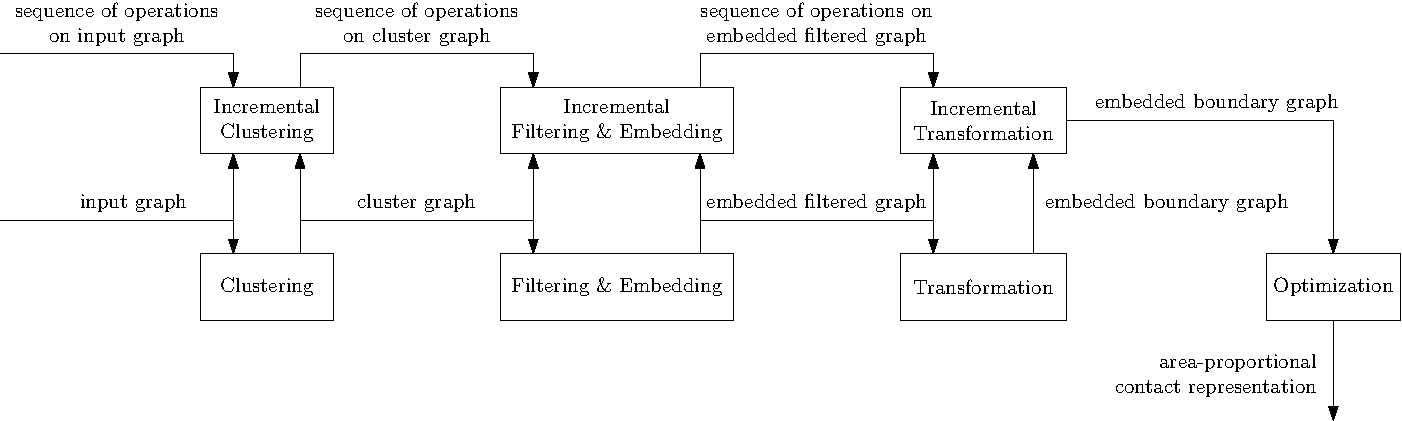
\includegraphics[width=0.9\textwidth]{Resources/DynamicPipeline.pdf}
	\caption{Overview of the algorithmic pipeline for dynamic input graphs.}
	\label{fig:dynamic-pipeline}
\end{figure}

The incremental versions of the clustering, filtering and embedding, and transformation phases propagate the incremental changes through the pipeline by adapting the operations for the different intermediate graphs: The incremental clustering phase tells us what effects a change of the input graph, as expressed by a sequence of operations on said graph, has on its cluster graph. The incremental filtering and embedding phase then tells us how those changes of the cluster graph in turn affect the embedded filtered graph. Eventually, the incremental transformation phase outputs an embedded boundary graph for the embedded filtered graph with the respective operations applied.

All of these phases tell us how to modify the graph output by their non-incremental counterparts using a sequence of operations or output a modified version of said graph directly. Note that a sequence of operations is only meaningful in combination with a graph that these operations can be applied to. However, we don't allow the incremental clustering and filtering \& embedding phases to output the intermediate graphs themselves. This would open us up to the possibility of the sequences of operations being incompatible with the graphs produced by the pipeline earlier. Recall that we already ran through the pipeline at least once and have a contact representation and intermediate products for the original input graph, and we now want to find out how changes of the original input graph translate to changes of the intermediate products and the eventual contact representation. We therefore provide the output graphs of the non-incremental phases as additional input to their incremental counterparts such that the incremental phases can tailor their output to whatever the pipeline has produced for earlier versions of the input graph.

The eventual optimization phase doesn't need to be adjusted for the dynamic case \emdash{} it simply obtains its input from the incremental transformation phase rather than from the regular transformation phase. Instead of optimizing a polygonal contact representation produced from an embedded filtered graph from scratch, it improves upon a contact representation that has previously been optimized and had a couple of tweaks made to it afterwards.

Extending the pipeline to allow the propagation of small, incremental changes of the input graph has numerous benefits other than the ability to preserve the viewer's mental map:
%
\begin{itemize}
	\item It allows highly efficient implementations of the incremental parts of the pipeline as only the aspects that have actually changed in the input graph or intermediate products need to be processed and incorporated further along the pipeline.
	\item It makes the dynamic pipeline highly parallelizable: when a later phase is processing changes, an earlier phase can already start processing new changes independently. For iterative implementations of the optimization phase this benefit is even greater, as dynamic updates can be incorporated at any point during the optimization, even if the optimization has not yet converged.
	\item It efficiently supports dynamic input in an online setting, \ie{} a setting in which the incremental changes aren't known in advance, for example when visualizing live data.
\end{itemize}

Because the dynamic pipeline is only able to incorporate a predefined class of operations, we must ensure that we can create any version of the input graph by applying some sequence of operations to the initial version of said graph, \ie{}
%
\begin{equation*}
	\forall G_i \colon \exists n \in \mathbb{N} \colon \exists (\text{op}_i)_{i=1}^{n_i} \colon \quad G_i = \text{apply}((\text{op}_i)_{i=1}^{n_i}, G_0),
\end{equation*}
%
where $\text{apply}(\cdot, G_0)$ applies a sequence of operations to the graph $G_0$. Otherwise it might not be possible to adapt the produced contact representation for a later version of the input graph.

We shall therefore support the following class of operations on the input graph:
%
\begin{itemize}
	\setlength\itemsep{-0.5em}
	\item add a vertex with arbitrary adjacencies
	\item remove a vertex and all its incident edges
	\item add a set of edges
	\item remove a set of edges
\end{itemize}
%
By applying a sequence of these primitive operations we can clearly turn an arbitrary graph $G_0 \coloneqq (V_0, E_0)$ into any other graph $G_i \coloneqq (V_i, E_i)$. Finding such a sequence for a pair of graphs $(G_0, G_1)$ is trivial: we can first remove vertices $V_0 \setminus V_1$ and edges $E_0 \setminus E_1$ and then add vertices $V_1 \setminus V_0$ and edges $E_1 \setminus E_0$.

Many real-world applications, such as the visualization of a dynamic opinion network from \cref{sect:motivation}, produce such a sequence of operations directly. For applications that don't, we can trivially prepend a phase that takes two versions of the input graph, the original version $G_0$ and an updated version $G_i$, computes a valid sequence of operations that turns $G_0$ into $G_i$ as described above, and feeds the original input graph and the sequence of operations to the incremental clustering phase.

\clearpage
\section{Incremental Clustering}
\label{sect:incremental-clustering}

The incremental clustering phase translates changes of the input graph to changes of its cluster graph: it takes a sequence of operations that was applied to a previous version of the input graph and its cluster graph as input and outputs a (potentially empty) sequence of operations to be applied to the cluster graph:

\begin{figure}[H]
	\centering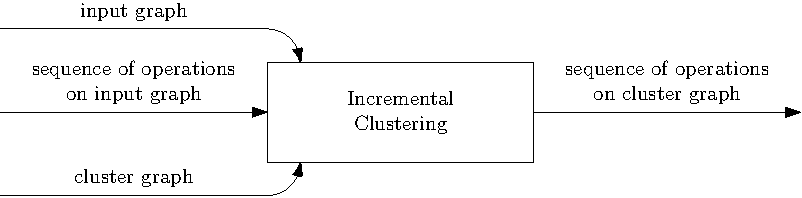
\includegraphics[width=0.8\textwidth]{Resources/DynamicPipeline-IncrementalClustering.pdf}
	\caption{Input and output of the incremental clustering phase.}
	\label{fig:dynamic-pipeline-incremental-transformation}
\end{figure}

The cluster graph of the previous version of the input graph is needed because the output sequence is tailored to a specific cluster graph. It has to be specified as input rather than being part of the output because we want to continue propagating the changes through the pipeline and apply it to a product of a non-incremental phase eventually. If we didn't specify these products as input to the incremental phases, the sequence of operations might not be compatible with the products of the non-incremental phases.

We assume that in concrete implementations, the cluster graph preserves enough information about the input graph to allow for incremental clustering. For example, the cluster graph might keep track of which vertices of input graph its clusters contain.
\todo{Or do we want to formalize that with explicit mathematical definitions of cluster graph etc.?}

The following operations on the cluster graph can be output and are sufficient to turn any cluster graph into a different one:
%
\begin{itemize}
	\setlength\itemsep{-0.5em}
	\item change a vertex' weight
	\item change an edge's weight
	\item add a vertex with arbitrary weight and edge weights to existing vertices
	\item remove a vertex
\end{itemize}
%
Note that because the cluster graph is a complete graph, we are not allowed to add or remove individual edges and adding a new vertex to the cluster graph implicitly adds edges to all existing vertices.

\clearpage
\section{Incremental Filtering and Embedding}
\label{sect:incremental-filtering-and-embedding}

The incremental filtering and embedding phase continues propagating the changes and translates changes of the cluster graph to changes of its filtered graph embedding: it takes a cluster graph, a sequence of operations to be applied to the cluster graph, and the embedded filtered graph of the cluster graph and outputs a sequence of operations that, when applied to the embedded filter graph, makes it an embedded filter graph of the cluster graph with the operations applied.

\begin{figure}[H]
	\centering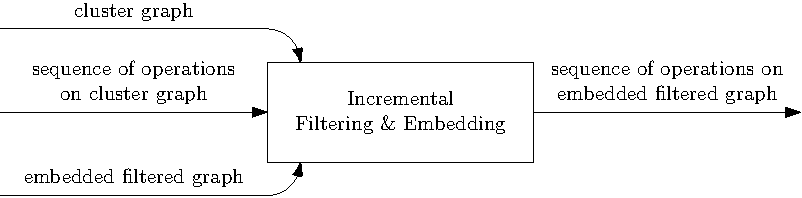
\includegraphics[width=0.9\textwidth]{Resources/DynamicPipeline-IncrementalFilteringAndEmbedding.pdf}
	\caption{Input and output of the incremental filtering and embedding phase.}
	\label{fig:dynamic-pipeline-incremental-filtering-and-embedding}
\end{figure}

The pipeline supports the following operations:
%Supported operations on embedded filtered graph:
%
\begin{itemize}
	\item \textbf{Change vertex or edge weight:}
	\item \textbf{Add vertex in an internal face:} with arbitrary weight inside an inner face (and connect it to the three vertices of the triangle)
	\item \textbf{Add vertex in outer face:} adjacent to 2 or more vertices on outer face that lie on simple path
	\item \textbf{Remove internal vertex:} of degree 3
	\item \textbf{Add edge on outer face:}
	\item \textbf{Remove edge on outer face:} without violating 2-connectedness and internal triangulatedness
	\item \textbf{Flip internal edge:}
\end{itemize}

\clearpage
\section{Incremental Transformation to Dual}
\label{sect:incremental-transformation-to-dual}

\lipsum

\begin{figure}[H]
	\centering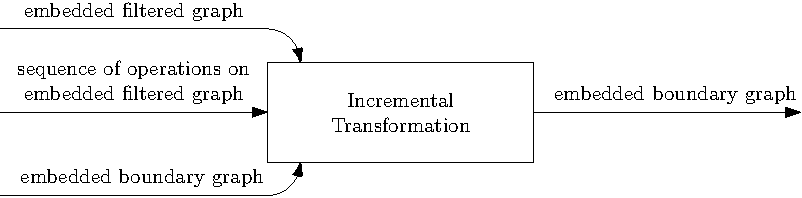
\includegraphics[width=0.9\textwidth]{Resources/DynamicPipeline-IncrementalTransformation.pdf}
	\caption{Input and output of the incremental transformation phase.}
	\label{fig:dynamic-pipeline-incremental-transformation}
\end{figure}

Supported operations translate 1 to 1 from embedded filtered graph:
%
\begin{itemize}
	\item xxx. replace vertex with face. replace edge with adjacency.
\end{itemize}

